\documentclass[parskip]{scrartcl}
\usepackage[margin=15mm,landscape]{geometry}
\usepackage{tikz}
 \usetikzlibrary{calc}

\begin{document}

\begin{figure}
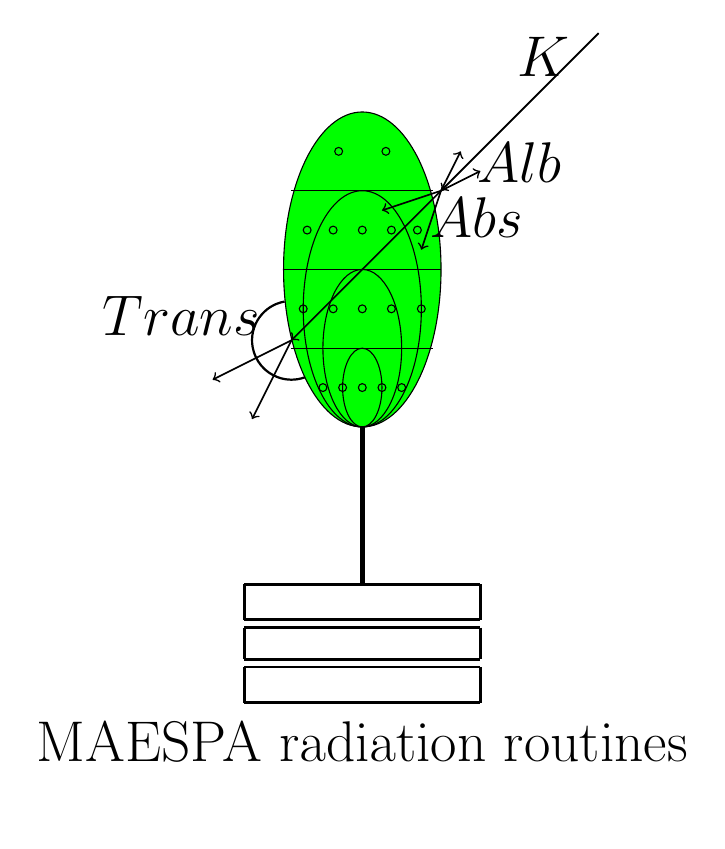
\begin{tikzpicture}

\coordinate (G1BCenter) at (0,0);
\coordinate (G1BCenter2) at (G1BCenter) ++(-1.0,-5.0);
\coordinate (soilstore) at (G1BCenter) ++ (0,-2.2);
    
	% stem of MAESPA tree   
	\draw[line width=2pt] (G1BCenter2)  -- ++(0,-2)  ;
	% and tree
	\draw[fill=green] (G1BCenter2) ++(0,2) ellipse (1cm and 2cm);
	%ellipses inside of tree
	\draw (G1BCenter2)  ++(0,1.5) ellipse (.75cm and 1.5cm);
	\draw (G1BCenter2)  ++(0,1) ellipse (.5cm and 1cm);
	\draw (G1BCenter2)  ++(0,.5) ellipse (.25cm and .5cm);
	%draw lines across tree
	\draw (G1BCenter2)  ++(0,1)  -- ++(-.9,0)  ;
	\draw (G1BCenter2)  ++(0,1)  -- ++(+.9,0)  ;
	
	\draw (G1BCenter2)  ++(0,2)  -- ++(-1.0,0)  ;
	\draw (G1BCenter2)  ++(0,2)  -- ++(+1.0,0)  ;
	
	\draw (G1BCenter2)  ++(0,3)  -- ++(-.9,0)  ;
	\draw (G1BCenter2)  ++(0,3)  -- ++(+.9,0)  ;
	%draw small grid circles
	\draw (G1BCenter2)  ++(.3,3.5) ellipse (.05cm and 0.05cm);
	\draw (G1BCenter2)  ++(-.3,3.5) ellipse (.05cm and 0.05cm);
	
	\draw (G1BCenter2)  ++(.0,2.5) ellipse (.05cm and 0.05cm);
	\draw (G1BCenter2)  ++(-.37,2.5) ellipse (.05cm and 0.05cm);
	\draw (G1BCenter2)  ++(.37,2.5) ellipse (.05cm and 0.05cm);
	\draw (G1BCenter2)  ++(.7,2.5) ellipse (.05cm and 0.05cm);
	\draw (G1BCenter2)  ++(-.7,2.5) ellipse (.05cm and 0.05cm);
	
	\draw (G1BCenter2)  ++(.0,1.5) ellipse (.05cm and 0.05cm);
	\draw (G1BCenter2)  ++(-.37,1.5) ellipse (.05cm and 0.05cm);
	\draw (G1BCenter2)  ++(.37,1.5) ellipse (.05cm and 0.05cm);
	\draw (G1BCenter2)  ++(-.75,1.5) ellipse (.05cm and 0.05cm);
	\draw (G1BCenter2)  ++(.75,1.5) ellipse (.05cm and 0.05cm);
	
	\draw (G1BCenter2)  ++(.0,0.5) ellipse (.05cm and 0.05cm);
	\draw (G1BCenter2)  ++(-.25,0.5) ellipse (.05cm and 0.05cm);
	\draw (G1BCenter2)  ++(.25,0.5) ellipse (.05cm and 0.05cm);
	\draw (G1BCenter2)  ++(-.5,0.5) ellipse (.05cm and 0.05cm);
	\draw (G1BCenter2)  ++(.5,0.5) ellipse (.05cm and 0.05cm);	
	
	%draw soil - hortz lines
	\draw[line width=1.0pt]  (G1BCenter)  ++(0,-2)  -- ++(-1.5,0)  ;
	\draw[line width=1.0pt]  (G1BCenter)  ++(0,-2)  -- ++(1.5,0)  ;
	
	\draw[line width=1.0pt]  (G1BCenter)  ++(0,-2.45)  -- ++(-1.5,0)  ;
	\draw[line width=1.0pt]  (G1BCenter)  ++(0,-2.45)  -- ++(1.5,0)  ;
	
	\draw[line width=1.0pt]  (G1BCenter)  ++(0,-2.55)  -- ++(-1.5,0)  ;
	\draw[line width=1.0pt]  (G1BCenter)  ++(0,-2.55)  -- ++(1.5,0)  ;
	
	\draw[line width=1.0pt]  (G1BCenter)  ++(0,-2.95)  -- ++(-1.5,0)  ;
	\draw[line width=1.0pt]  (G1BCenter)  ++(0,-2.95)  -- ++(1.5,0)  ;
	
	\draw[line width=1.0pt]  (G1BCenter)  ++(0,-3.05)  -- ++(-1.5,0)  ;
	\draw[line width=1.0pt]  (G1BCenter)  ++(0,-3.05)  -- ++(1.5,0)  ;
	
	\draw[line width=1.0pt]  (G1BCenter)  ++(0,-3.5)  -- ++(-1.5,0)  ;
	\draw[line width=1.0pt]  (G1BCenter)  ++(0,-3.5)  -- ++(1.5,0)  ;
	%draw soil - vert lines
	\draw[line width=1.0pt]  (G1BCenter)  ++(-1.5,-2) -- ++(0,-0.45) ;
	\draw[line width=1.0pt]  (G1BCenter)  ++(1.5,-2) -- ++(0,-0.45) ;
	
	\draw[line width=1.0pt]  (G1BCenter)  ++(-1.5,-2.55) -- ++(0,-0.40) ;
	\draw[line width=1.0pt]  (G1BCenter)  ++(1.5,-2.55) -- ++(0,-0.40) ;
	
	\draw[line width=1.0pt]  (G1BCenter)  ++(-1.5,-3.05) -- ++(0,-0.45) ;
	\draw[line width=1.0pt]  (G1BCenter)  ++(1.5,-3.05) -- ++(0,-0.45) ;	
	
	%k from sun
	\draw[arrows=->,line width=0.6pt] (G1BCenter)++(0,2)++(3.0,3.0) -- ++(-2.0,-2.0)   		 	node[font=\Huge,label={[xshift=1.3cm, yshift=1.2cm]\huge$K$}] 
{} ;
% 2 albedo arrows
\draw[arrows=->,line width=0.6pt] (G1BCenter)++(0,2)++(3.0,3.0)++(-2.0,-2.0)  -- ++(0.5,0.25) node[font=\LARGE,label={[xshift=0.5cm, yshift=-0.4cm]\huge$Alb$}] 	{} ;	
\draw[arrows=->,line width=0.6pt] (G1BCenter)++(0,2)++(3.0,3.0)++(-2.0,-2.0) -- ++(0.25,0.5) node[font=\Large,label={[xshift=0.5cm, yshift=-0.4cm]}] 	{} ;
% 2 abs arrows
\draw[arrows=->,line width=0.6pt] (G1BCenter)++(0,2)++(3.0,3.0)++(-2.0,-2.0)  -- ++(-0.75,-0.25) node[font=\Large,label={[xshift=1.2cm, yshift=-0.6cm]\huge$Abs$}] 	{} ;	
\draw[arrows=->,line width=0.6pt] (G1BCenter)++(0,2)++(3.0,3.0)++(-2.0,-2.0) -- ++(-0.25,-0.75) node[font=\Large,label={[xshift=0.5cm, yshift=-0.4cm]}] 	{} ;

% k from sun through tree
\draw[arrows=->,line width=0.6pt] (G1BCenter)++(0,2)++(3.0,3.0) -- ++(-3.9,-3.9) 
%		node[font=\Large,label={[xshift=-1.7cm, yshift=-0.2cm]$K$}] 
		{} ;
	%\draw[red] (G1BCenter)++(0,2)++(3.0,3.0)++(-3.9,-3.9)  ellipse (.1cm and 0.1cm);	
	
\def\centerarc[#1](#2)(#3:#4:#5)% [draw options] (center) (initial angle:final angle:radius) 
{ \draw[#1] ($(#2)+({#5*cos(#3)},{#5*sin(#3)})$) arc (#3:#4:#5); }

%draw ray exits
%\coordinate (treeexit) at (G1BCenter)++(0,0)++(3.0,3.0)++(-3.9,-3.9);
\centerarc[thick](-0.90,1.10)(100:290:0.5);
%\draw[red] (-0.90,1.10)  ellipse (.1cm and 0.1cm);	

%transmission
\draw[arrows=->,line width=0.6pt] (-0.90,1.10)  -- ++(-1.0,-0.5) node[font=\Large,label={[xshift=-0.4cm, yshift=0.3cm]\huge$Trans$}] 	{} ;	
\draw[arrows=->,line width=0.6pt] ((-0.90,1.10) -- ++(-0.5,-1.0) node[font=\Large,label={[xshift=0.5cm, yshift=-0.4cm]}] 	{} ;
	
%\draw[red]  (G1BCenter)++(0,2)++(3.0,3.0)++(-3.9,-3.9)   arc (180:270:2cm);	
		
%\draw[arrows=->,line width=0.6pt] (G1BCenter)++(-7.0,-7.0) -- ++(0.5,0.25) node[font=\Large,label={[xshift=0.5cm, yshift=-0.4cm]$Albedo$}] 	{} ;	
%\draw[arrows=->,line width=0.6pt] (G1BCenter)++(-7.0,-7.0) -- ++(0.25,0.5) node[font=\Large,label={[xshift=0.5cm, yshift=-0.4cm]}] 	{} ;	
 			 			

	 		
\draw[] (0.00,-4.50) node[font=\Large,label={[xshift=0.0cm, yshift=0.0cm]\huge MAESPA radiation routines}] 	{} ;	
			 		 
    
\end{tikzpicture}
\end{figure}



\end{document}